%!TEX root = uw-ethesis.tex
% chktex-file 46 (ignore warnings about $...$)
% chktex-file 24 (ignore \label warning)
\chapter{Preliminaries}\label{chap:prelims}

In this chapter, we introduce some core background concepts that arise throughout the thesis. First, we detail the notation and specify the semantics of a our choice of temporal logic, \mucalc{}, and provide the model checking tools necessary to use it. A description of the incremental kinodynamic planning algorithm \gls{sst}* follows, along with a description of the various functions used to implement the planning algorithm. This is contrasted with \gls{fmt}, which is another motion planning algorithm that is not incremental.


%%%%%%%%%%%%%%%%%%%%%%%%%%%%%%%%%%%%%%%%%%%%%%%%%%%%%%%%%%%%%%%%%%%%%%%%%%%%%%%%
%%%%%%%%%%%%%%%%%%%%%%%%%%%%%%%%%%%%%%%%%%%%%%%%%%%%%%%%%%%%%%%%%%%%%%%%%%%%%%%%
\section{\texorpdfstring{$\mu$-Calculus}{mu-Calculus}}
%%%%%%%%%%%%%%%%%%%%%%%%%%%%%%%%%%%%%%%%%%%%%%%%%%%%%%%%%%%%%%%%%%%%%%%%%%%%%%%%
%%%%%%%%%%%%%%%%%%%%%%%%%%%%%%%%%%%%%%%%%%%%%%%%%%%%%%%%%%%%%%%%%%%%%%%%%%%%%%%%

We begin by defining the syntax and semantics of the full, modal \mucalc{}. A simple example Kripke structure is provided to build some intuition surrounding the notation and meaning of some common \mucalc{} formulas. We then describe a fragment of \mucalc{} called deterministic \mucalc{}, which we will be using for the motion planning procedure in \autoref{chap:sstpaper}. Finally, we present many examples of typical deterministic \mucalc{} formulas, describing how to parse and thoroughly understand each one.



%%%%%%%%%%%%%%%%%%%%%%%%%%%%%%%%%%%%%%%%%%%%%%%%%%%%%%%%%%%%%%%%%%%%%%%%%%%%%%%%

\subsection{\texorpdfstring{Modal $\mu$-Calculus}{Modal mu-Calculus} }
First, an atomic proposition is a declarative statement that is either true or false, and which cannot be further split into smaller statements. An example of an atomic proposition might be ``in free space'', where a state satisfies the atomic proposition if and only if it lies in the defined free space for a problem. On the other hand, the statement ``in free space AND not in goal region'' is not an atomic proposition, as it can be further deconstructed into the simpler statements ``in free space'' and ``in goal region''. As this example demonstrates, more complex statements use logical connectives such as conjunction ($\land$, logical AND), disjunction ($\lor$, logical OR), and negation ($\lnot$, logical NOT). We will also be using the modal operators $\Diamond$ and $\square$, and the symbols $\mu$ and $\nu$ as least and greatest fixed point operators, respectively. Definitions for these fixed point operators will be provided.

Let $\Pi$ be the set of atomic propositions, and let $\Var$ be the set of variables. Then we define the following structure as in~\cite{Karaman2009}.
\begin{defn}\label{defn:kripke}
    A \emph{Kripke structure} $K$ over the set of atomic propositions $\Pi$ is a tuple $(S,S_0,R,\mathcal{L})$ where $S$ is a finite set of states, $S_0 \subseteq S$ is a set of initial states,  $R \subseteq S \times S$ is a binary relation which indicates a means of transiting from one state to another (usually represented as the edges in a directed graph), and $\mathcal{L}:S \to 2^\Pi$ is a labeling function, mapping each state to the subset of propositions that it satisfies.
\end{defn}

In essence, a Kripke structure is a graph with edges representing available transitions between nodes, which represent states that have been added to the graph via some sampling scheme. The distinction to be made between a Kripke structure and any other graph representation is that every node on the graph has an associated label which defines which atomic propositions that node satisfies. \autoref{fig:kripke} is an example of graph that could represent a Kripke structure.
The set of states, $S$, is represented by the nodes of the graph, the set of initial states is given by the singleton containing the bottom-left node, and the set of relations is represented by the edges. Define $\pi_f$ to be the atomic proposition ``in free space'', $\pi_g$ to mean ``in goal'', and $\pi_o$ to mean ``in obstacle''. The labeling function would then simply specify, for every node, the subset of $\Pi = \{ \pi_f, \pi_g, \pi_o \}$ that it satisfies.

\begin{figure}[!ht]
    \begin{center}
        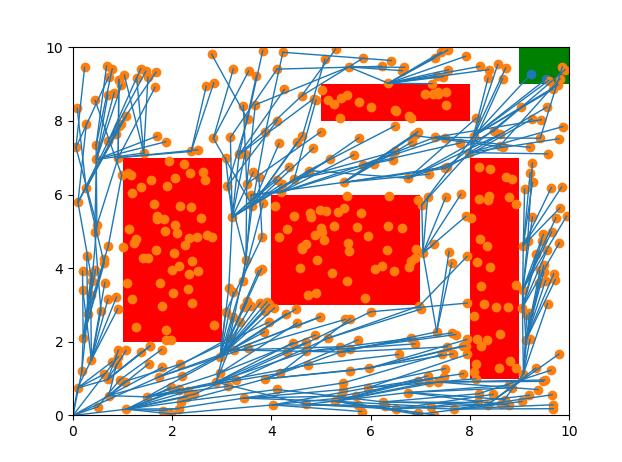
\includegraphics[width=0.85\textwidth]{./figures/kripke_example}
    \end{center}
    \caption[Example of a Kripke structure]{Example of a Kripke structure, with obstacles shown in red, free space shown in white, and the goal set shown in green.}
\label{fig:kripke}
\end{figure}


\noindent Define the set of valid \mucalc{} formulas ($L_\mu$) inductively, as follows:
\begin{itemize}
    \item the symbols \true{} and \false{} are formulas;
    \item every $p \in \Pi$ and $X \in \Var$ is a formula;
    \item if $\phi,\psi$ are formulas, then $\lnot \phi$, $\phi \land \psi$, and $\phi \lor \psi$ are also formulas;
    \item if $\phi$ is a formula then $\Diamond \phi$ and $\square \phi$ are formulas;
    \item if $\phi[X]$ is a formula where $\phi[X]$ is syntactically monotone in $X$, then $\mu X.\phi$ and $\nu X.\phi$ are formulas.
\end{itemize}
As in~\cite{Gurfinkel2004}, we write $\phi[X]$ to indicate that $\phi$ may contain an occurrence of $X$.

Next, we state definitions that will prove to be useful in the discussion of model checking for our chosen fragment of \mucalc{}, deterministic \mucalc{}, which will be seen in \autoref{prelims:deterministic_mucalc}.

\begin{defn}
    Given a \mucalc{} specification, $\phi$, we say that a variable $X$ is {\em positive\/} (respectively, {\em negative\/}) if it occurs under the scope of an even (respectively, odd) number of negations in $\phi$.
\end{defn}

\begin{defn}
    A subformula $X$ is {\em pure\/} in \mucalc{} specification $\phi$ if all of its occurrences have the same polarity (i.e., all occurrences of $X$ are positive or all occurrences of $X$ are negative).
\end{defn}

\begin{defn}
    The formula $\phi[X]$ is {\em syntactically\/monotone} in $X$ if and only if $X$ occurs with pure polarity in $\phi$.
\end{defn}


\mucalc{} formulas are interpreted with respect to a Kripke structure $K = (S,S_0,R,\mathcal{L})$ and an {\em environment\/} (also called an {\em evaluation\/}), $e: \Var \to 2^S$, which initializes (i.e., assigns a subset of $S$ to) each free variable, where a free variable is defined in the usual sense and a variable is otherwise said to be bound by a fixed point operator. For every $L_\mu$ formula $\phi$, given a Kripke structure, $K$, define $\brackets{\phi}_K^e \subseteq S$ to be the set of states of $S$ satisfying proposition $\phi$ (note that the subscript $K$ is often omitted when the Kripke structure being used is clear, and the superscript $e$ is omitted when $\phi$ contains no free variables). The semantics of the formulas is determined inductively by the following, where $p \in \Pi$, $X \in \Var$, and $\phi, \psi \in L_\mu$ are arbitrary formulas~\cite{Wilke2001}.

\begin{tabular}{l}
    $\lb \false \rb_K = \emptyset$ \\
    $\lb \true \rb_K = S$ \\
    $\brackets{p}_K = \{s \in S : p \in \mathcal{L}(s) \}$ \\    
    $\lb \lnot p \rb_K = S \setminus \lb p \rb$ \\
    $\brackets{\phi \lor \psi}_K^e = \brackets{\phi}_K^e \cup \brackets{\psi}_K^e $ \\ 
    $\brackets{\phi \land \psi}_K^e = \brackets{\phi}_K^e \cap \brackets{\psi}_K^e $ \\
    $\brackets{\Diamond \phi}_K^e = \Pree{\phi}$ \\
    $\brackets{\square \phi}_K^e = \Prea{\phi}$ \\
    $\brackets{\mu X. \phi}_K^e = \bigcap \{ A \subseteq S : \brackets{\phi}_K^{e[X \leftarrow A]} \subseteq A \}$ \\
    $\brackets{\nu X. \phi}_K^e = \bigcup \{ A \subseteq S : \brackets{\phi}_K^{e[X \leftarrow A]} \supseteq A \}$
\end{tabular}

\vspace*{2.2mm}
\noindent
The existential and universal {\em predecessor\/} functions $\text{Pre}_{K,\ \cdot}^e:L_\mu \to S$ map a \mucalc{} formula to the set of states which immediately precede (i.e., have transitions to) states satisfying said formula in the Kripke structure $K$ and under evaluation $e$:
\begin{align*}
    \Pree{\phi} &:= \{ s \in S : \exists s' \in S \ \text{s.t.} \ (s,s') \in R \land s' \in \brackets{\phi}_K^e\} \\
    \Prea{\phi} &:= \{ s \in S : \forall s' \in S, (s,s') \in R \implies s' \in \brackets{\phi}_K^e\}.
\end{align*}

In words, $\true{} = (p \lor \lnot p)$ holds for all states in $S$, and $\false{} = (p \land \lnot p)$ does not hold for any state in $S$; disjunction and conjunction of formulas is equivalent to the union and intersection of the sets which satisfy them, respectively; $\Diamond$ is the {\em existential\/successor} (or ``next'') operator, and $\square$ is the {\em universal\/successor} operator; lastly, $\mu$ and $\nu$ are the {\em least\/} and {\em greatest\/fixed-point} operators, respectively, where $e[X \leftarrow A]$ is a modified evaluation function which maps $X$ to $A$, i.e., $e[X \leftarrow A](X) = A$. To help build a more intuitive understanding of these last four semantic definitions, a simple example is provided (\autoref{mucalc_example}).

\begin{figure}[!hb]
    \centering
    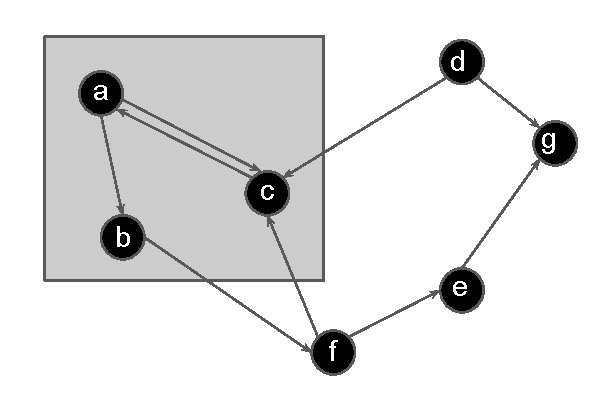
\includegraphics[width=0.6\textwidth]{./figures/mucalc_example}
    \caption[$\mu$-Calculus semantics example]{$\mu$-Calculus semantics \autoref{mucalc_example}.}
\label{fig:mucalc_example}
\end{figure}

\begin{exmp}\label{mucalc_example}
This example illustrates the semantics presented above. Refer to \autoref{fig:mucalc_example}.\\
Define atomic proposition $p$ to be the boolean value corresponding to ``in gray region''. We can specify the labeling function for each node, writing $\mathcal{L}(s_p) = \{p\}$ for nodes $s_p \in \{a, b, c\}$, and $\mathcal{L}(s) = \emptyset$ for nodes $s \in \{d, e, f, g \}$. Note that the environment superscript $e$ is omitted as we are not using any free variables.

\begin{tabular}{l}\label{table:modal_mucalc_syntax}
    $\brackets{p}_K = \{s \in S : p \in \mathcal{L}(s) \} = \{a, b, c\}$ \\    
    $\lb \lnot p \rb_K = S \setminus \lb p \rb$ = \{d, e, f, g \} \\
    $\brackets{\Diamond p}_K = \Pree{p} = \{a, c, d, f\}$ \\
    $\brackets{\square p}_K = \Prea{p}$ = \{a, c\} \\
    $\brackets{\mu X.(p \lor \Diamond X)}_K = \bigcap \{ A \subseteq S : \brackets{\phi}_K^{e[X \leftarrow A]} \subseteq A \} = \{ a,b,c,d,f \}$ \\
    $\brackets{\nu X.(p \land \Diamond X)}_K = \bigcup \{ A \subseteq S : \brackets{\phi}_K^{e[X \leftarrow A]} \supseteq A \} = \{ a, c \}$
\end{tabular}

\begin{itemize}
    \item $\brackets{p}_K$ is the set of nodes satisfying $p$ (nodes in the gray region).
    \item $\lb \lnot p \rb_K$ is the complement of $\brackets{p}_K$ in $S$ (nodes that are not in the gray region).
    \item $\brackets{\Diamond p}_K$ contains those nodes that have a transition to a node in the gray region.
    \item $\brackets{\square p}_K$ contains only nodes such that \emph{every} transition leads to a node in the gray region.
    \item $\brackets{\mu X.(p \lor \Diamond X)}_K$ is the \emph{reachability} specification which determines whether there exists a sequence of transitions reaching a state satisfying $p$ (see \autoref{prelims:spec_examples}). In this case, the resulting set consists of the nodes that are in the gray region \emph{or} that can follow transitions to eventually reach a node in the gray region.
    \item $\brackets{\nu X.(p \land \Diamond X)}_K$ is the \emph{safety} specification which determines whether there exists a sequence of transitions guaranteeing that proposition $p$ is always satisfied (see \autoref{prelims:spec_examples}). In this case, the resulting set consists of the nodes that are in the gray region \emph{and} can always take a transition to a node that is also in the gray region. 
\end{itemize}
\end{exmp}

In order to develop a means of evaluating expressions containing fixed-point operators, we rely on the Tarski-Knaster theorem from set theory. The next section introduces some definitions before stating the required theorem.





%%%%%%%%%%%%%%%%%%%%%%%%%%%%%%%%%%%%%%%%%%%%%%%%%%%%%%%%%%%%%%%%%%%%%%%%%%%%%%%%

\subsection{Tarski-Knaster Theorem}

The Tarski-Knaster fixed-point theorem (\autoref{thm:tarski}) we introduce in this section makes an important statement about complete lattices and their fixed-points~\cite{Tarski1955}. We make use of this theorem to formulate an algorithm which computes the least or greatest fixed points for the set of states satisfying a \mucalc{} proposition containing a least or greatest fixed point operator. Note that if a proposition does not contain fixed point operators or the existential successor operator, it is easy to evaluate the set of states satisfying such a proposition. We begin by defining the necessary concepts.

\begin{defn}
    Let $(X, \leq)$ be a partially ordered set, and let $A \subseteq X$. Then $\bigvee A$ ($\bigwedge A$) denotes the least upper bound (respectively, greatest lower bound) of $A$ with respect to $\leq$, if it exists. We say that $X$ is a {\em complete\/lattice} if, for every $A \subseteq X$, then both $\bigvee A$ and $\bigwedge A$ exist in $X$.
\end{defn}

\begin{exmp}\label{ex_complat}
Consider $(\mathcal{P}(X), \subseteq)$ for any set $X$, where $\mathcal{P}(X)$ denotes the power set of $X$. Note that $\forall A \subseteq \mathcal{P}(X), \ \bigvee A = \bigcup A$, since the union of all the elements of $A$ gives the smallest set which completely contains the elements of each subset in $A$, and this union must be an element of $\mathcal{P}(X)$. Similarly, $\bigwedge A = \bigcap A \in \mathcal{P}(X)$. Thus, $(\mathcal{P}(X), \subseteq)$ is a complete lattice.
\end{exmp}

\begin{defn}
Let $(A, \leq_A)$ and $(B, \leq_B)$ be partially ordered sets. A function $f : A \to B$ is {\em monotone\/} if $a_1 \leq_A a_2 \implies f(a_1) \leq_B f(a_2)$.\\
A point $a \in A$ is a {\em fixed\/point} of a function $f: A \to B$ if $f(a) = a$, and we denote the set of all fixed points of $f$ by $\textsc{fix}(f)$.
\end{defn}

\begin{thm}\label{thm:tarski}
    \text{\normalfont(Tarski-Knaster Fixed Point Theorem)}~\\
    Let $\mathbb{L}$ be a complete lattice and let $F: \mathbb{L} \to \mathbb{L}$ be monotone. Then
    \begin{enumerate}
    \item $\bigvee \{ x \in \mathbb{L} \ \vert \ x \leq F(x) \} \in \textsc{fix}(F)$,
    \item $\bigwedge \{ x \in \mathbb{L} \ \vert \ F(x) \leq x \} \in \textsc{fix}(F)$, and
    \item $\textsc{fix}(F)$ is a complete lattice.
    \end{enumerate}
\end{thm}

\begin{proof}~\\
    Let $\mu F := \{ u \in \mathbb{L} \ \vert \ u \leq F(u) \}$, and
    let $\zeta = \bigvee \mu F$ ($\zeta$ exists since $\mu F \subseteq \mathbb{L}$, a complete lattice).
    For all $u \in \mu F$, $u \leq \zeta$, so $u \leq F(u) \leq F(\zeta)$, by monotonicity.
    Thus, $F(\zeta)$ is an upper bound for $\mu F$, and $\zeta$ is the least upper bound, so $\zeta \leq F(\zeta)$.
    By monotonicity, $F(\zeta) \leq F(F(\zeta))$, so $F(\zeta) \in \mu F$. This implies that that $F(\zeta) \leq \zeta$.
    Therefore, $\zeta = F(\zeta) \in \textsc{fix}(F)$.
    A similar argument can be made for $\bigwedge \{ u \in \mathbb{L} \ \vert \ F(u) \leq u \}$.

    Now we show that an arbitrary subset $A \subseteq \textsc{fix}(F)$ has a least upper bound and a greatest lower bound, thereby proving $\textsc{fix}(F)$ is a complete lattice.
    Define $a:=\bigvee A$, and $1_\mathbb{L} = \bigvee \mathbb{L}$.
    Consider the interval $[a,1_\mathbb{L}] := \{ x \in \mathbb{L} \ \vert \ a \leq x \leq 1_\mathbb{L} \}$, which is a complete lattice.
    Then if $A$ has a least upper bound in $\textsc{fix}(F)$, it must lie in $[a,1_\mathbb{L}]$.
    Note that it suffices to show that $F$ can be restricted to act as a monotone function
    $F:[a,1_\mathbb{L}] \to [a,1_\mathbb{L}]$, so that we may apply the first result: a monotone function on the complete lattice $[a,1_\mathbb{L}]$ has a least fixed point, and this point is therefore the least upper bound of $A \subseteq \textsc{fix}(F)$.
    Let $x \in A$. Then $x \leq a$ and $x = F(x) \leq F(a) = a$ by monotonicity, so $a \leq F(a)$.
    Letting $y \in [a,1_\mathbb{L}]$, we can see that $a \leq y$ and $a = F(a) \leq F(y) \leq 1_\mathbb{L}$ by monotonicity.
    This implies $F(y) \in [a,1_\mathbb{L}]$, so we conclude that $F([a,1_\mathbb{L}]) \subseteq [a,1_\mathbb{L}]$ which further implies that we may restrict the domain and co-domain, $F: [a,1_\mathbb{L}] \to [a,1_\mathbb{L}]$.
    We have thus shown that an arbitrary subset $A \subseteq \textsc{fix}(F)$ has a least upper bound in $\textsc{fix}(F)$. It is true for all lattices $\mathbb{L}$ that if every sublattice $S \subseteq \mathbb{L}$ has a least upper bound $\bigvee S$, then $S$ has a greatest lower bound defined by
    \[\bigwedge S = \bigvee \left( \bigcap\limits_{s \in S} \{ x \in \mathbb{L}: x \leq s \} \right).\]
    Therefore, $\textsc{fix}(F)$ is a complete lattice.
\end{proof}

We will use this theorem to perform model checking over a Kripke structure on propositions with a fixed point operator $\phi = \sigma X.\psi$, where we use $\sigma$ as a generic symbol to represent either $\mu$ or $\nu$.

\begin{cor}\label{cor:tarskialg}
    Let $K = (S,S_0,R,\mathcal{L})$ be a Kripke structure, $e: \Var \to 2^S$ be an evaluation, and $\phi \in L_1$ be a deterministic \mucalc{} formula. Define $Q_i^\mu$ and $Q_i^\nu$ recursively as follows:
    \vspace{2mm}\\
    % chktex-file 44  (disables warning for vertical line in table)
    \begin{tabular}{l | l}
        $Q_0^\mu = \emptyset$   
            & $Q_0^\nu = S$\\
        $Q_i^\mu = \brackets{\phi}_K^{e[X \leftarrow Q_{i-1}^\mu]}$ 
            & $Q_i^\nu = \brackets{\phi}_K^{e[X \leftarrow Q_{i-1}^\nu]}$
    \end{tabular}\\

    \noindent then 
    \begin{enumerate}[label = (\roman*)]   
        \item $\forall i \in \mathbb{N},\ Q_{i-1}^\mu \subseteq Q_i^\mu$ and $Q_i^\nu \subseteq Q_{i-1}^\nu$,
        \item $\exists n,m \in \mathbb{N}$ such that $Q_{n-1}^\mu = Q_n^\mu$, $Q_{m-1}^\nu = Q_m^\nu$, and
        \item $Q_n^\mu = \brackets{\mu X.\phi}_K^e$, $Q_m^\nu = \brackets{\nu X.\phi}_K^e$.
    \end{enumerate}
\end{cor}

\sref{Corollary}{cor:tarskialg} presents an intuitive algorithm for finding the least and greatest fixed points satisfying a given \mucalc{} proposition with fixed point operators. Note that the complete lattice in question is the power set of the set of states ordered by set inclusion, ${(\mathcal{P}(S), \subseteq)}$, as in \autoref{ex_complat}. The proof relies on the fact that deterministic \mucalc{} propositions are inherently {\em syntactically\/monotone} and therefore {\em monotone\/} in their variables~\cite{Gurfinkel2004}, as negation is allowed only on atomic propositions. This implies that for any formula of the form $\sigma X.\psi[X]$, $A \subseteq B$ implies $\brackets{\psi}_K^{e[X \leftarrow A]} \subseteq \brackets{\psi}_K^{e[X \leftarrow B]}$. Summarizing the algorithm, to evaluate $\brackets{\mu X.\psi}_K^e$, it suffices to set $Q_1^\mu$ to be the set of states satisfying the formula $\psi$ where $X = Q_0^\mu$ is initialized to be the empty set. We then proceed inductively, letting each subsequent $Q_i^\mu$ be the result of finding the states which satisfy $\psi$ where $X$ is replaced by $Q_{i-1}^\mu$. After a finite number $n$ of iterations (since the set of states $S$ of a Kripke structure is finite, see~\autoref{defn:kripke}), a fixed point $Q_{n-1} = Q_n = \brackets{\mu X.\psi}_K^e$ will be reached. An analogous algorithm is applied when we wish to evaluate $\brackets{\nu X.\phi}_K^e$, where $Q_0^\nu = X$ is initialized to be $S$.






%%%%%%%%%%%%%%%%%%%%%%%%%%%%%%%%%%%%%%%%%%%%%%%%%%%%%%%%%%%%%%%%%%%%%%%%%%%%%%%%

\subsection{\texorpdfstring{Deterministic $\mu$-Calculus}{Deterministic mu-Calculus}}\label{prelims:deterministic_mucalc}

We will focus our efforts on a fragment of \mucalc{} called {\em deterministic\/\mucalc{}\/} which admits efficient model checking algorithms and is at least as expressive as the commonly used linear time temporal logics \gls{ltl} and \gls{ctl}~\cite{Karaman2009}. Deterministic \mucalc{} imposes some restrictions on syntax, notably that only atomic propositions may be negated, conjunction can only occur between a formula and an atomic proposition, and the universal successor operator $\square$ is omitted. We may write this syntax succinctly in Backus-Naur form as follows:
\[ 
\phi := p \ | \ \lnot p \ | \ X \ | \ p \land \phi \ | \ \lnot p \land \phi \ | \ \phi \lor \phi \ | \ \Diamond \phi \ | \ \mu X.\phi \ | \ \nu X. \phi
\]
where $p \in \Pi$ and $X \in \Var$. We denote the set of all deterministic $\mu$-calculus formulas by $L_1$. Note that by restricting negation to atomic propositions only, we ensure that every formula in $L_1$ is syntactically monotone in its variables.


%%%%%%%%%%%%%%%%%%%%%%%%%%%%%%%%%%%%%%%%%%%%%%%%%%%%%%%%%%%%%%%%%%%%%%%%%%%%%%%%




\subsection{Specification Examples}\label{prelims:spec_examples}

This section will introduce several examples of commonly used deterministic \mucalc{} specifications. Each example is named, described, and explained in detail to provide some intuition to the reader~\cite{Karaman2009}.

\begin{enumerate}[label = (\roman*)]
    \item \textbf{Reachability}: $\phi = \mu X.(p \lor \Diamond X)$\label{reachability_example} \\
        The reachability specification is used to ensure that the system eventually reaches a state which satisfies atomic proposition $p$. The resulting set $\brackets{\phi}_K^e$ is the {\em winning set}, that is, the set of all initial states for which the proposition $\phi$ holds. In this case, the winning set consists of states which satisfy $p$ or for which there exists a sequence of transitions in $R$ which lead to a state satisfying $p$. In the context of the Kripke structure $K = (S,S_0,R,\mathcal{L})$, we seek only to show that $S_0$ is contained in the winning set $\brackets{\phi}_K^e$.

        In this example, we look for the least fixed point because we will start with the empty set and grow through all states that satisfy $p$ or that can reach $\brackets{p}_K$ with one transition, then two transitions, and so on until the entire winning set is found. This process is guaranteed to terminate since the formula $(p \lor \Diamond X)$ is monotone ($\phi$ is a deterministic \mucalc{} formula), and since the Kripke structure contains finitely many states. Let us apply the algorithm from \sref{Corollary}{cor:tarskialg} to elucidate the procedure:
        \begin{align*}
            Q_0^\mu &= \emptyset \\
            Q_1^\mu &= \brackets{p \lor \Diamond X}_K^{e[X \leftarrow Q_0^\mu]} \\
                    &= \brackets{p}_K \cup \brackets{\Diamond X}_K^{e[X \leftarrow \emptyset]}\\
                    &= \brackets{p}_K \cup \Pree[{e[X \leftarrow \emptyset]}]{X} \\
                    &= \brackets{p}_K \cup \{ s \in S : \exists s' \in S \ \text{s.t.} \ (s,s') \in R   \land s' \in \emptyset \} \\
                    &= \brackets{p}_K\\
            Q_2^\mu &= \brackets{p \lor \Diamond X}_K^{e[X \leftarrow Q_1^\mu]} \\
                    &= \brackets{p}_K \cup \{ s \in S : \exists s' \in S \ \text{s.t.} \ (s,s') \in R \land s' \in \brackets{p}_K \}.
        \end{align*}
        This process continues until the least fixed point is reached. See \autoref{mucalc_example} for a concrete illustration of the reachability specification.

    \item \textbf{Safety}: $\phi = \nu X.(p \land \Diamond X)$\label{safety_example} \\
        We use the the term ``safety'' as this specification guarantees that a given atomic proposition will hold on some state trajectory; the atomic proposition may be concerned with being in an obstacle-free space, or it may ensure that constraints on speed or acceleration are observed, for instance. The formula $\phi$ will hold for all states which satisfy $p$ and which have transitions to states which will themselves satisfy $p$ and in turn have transitions to other states that will satisfy this same condition. For this reason, we start with the entire set of states, $S$, and repeatedly find intersections to narrow down the states until the greatest fixed point is reached.
        \begin{align*}
            Q_0^\nu &= S\\
            Q_1^\nu &= \brackets{p \land \Diamond X}_K^{e[X \leftarrow Q_0^\nu]} \\
                    &= \brackets{p}_K \cap \brackets{\Diamond X}_K^{e[X \leftarrow S]}\\
                    &= \brackets{p}_K \cap \{ s \in S : \exists s' \in S \ \text{s.t.} \ (s,s') \in R \land s' \in S\} \\
                    &= \brackets{p}_K\\
            Q_2^\nu &= \brackets{p \land \Diamond X}_K^{e[X \leftarrow Q_1^\nu]} \\
                    &= \brackets{p}_K \cap \{ s \in S : \exists s' \in S \ \text{s.t.} \ (s,s') \in R   \land s' \in \brackets{p}_K\} \\
            \vdots
        \end{align*}
        See \autoref{mucalc_example} for a concrete illustration of the safety specification.


    \item \textbf{Reaching a Region Safely}: $\phi = \mu X.(\lnot q \land (p \lor \Diamond X))$\\
        One way of combining the above two specifications is to ensure that a safety condition is met while trying to reach an objective. This specification is commonly used for motion planning problems, wherein a planner searches for a trajectory which avoids obstacles (represented by states satisfying $q$), and reaches a given goal (represented by states satisfying $p$). Obstacle avoidance is guaranteed by the conjunction of the usual reachability subformula with ${\lnot q}$ so that at each iteration, we keep only those states which satisfy the reachability criterion and are not obstacles.

    \item \textbf{Reaching a Safe Region}: $\phi = \mu X.((\nu Y.(p \land \Diamond Y)) \lor \Diamond X)$\\
    Another way to combine safety and reachability is the specification to reach a region whose states always satisfy a property $p$. The subformula ${\psi = \nu Y.(p \land \Diamond Y)}$ is identical to the safety specification listed above; $\psi$ is satisfied by all initial states which give rise to trajectories that always satisfy $p$. This safety specification is wrapped in the reachability specification ${\mu X.(\psi \lor \Diamond X)}$, meaning states which satisfy $\phi$ are either in the safe region already, or can reach the safe region using a finite number of transitions.

    \item \textbf{Ordering}: $\phi = \mu X.(q \lor (p \land \Diamond X))$\\
    In both \gls{ltl} and \gls{ctl}, there is a temporal operator \textsc{U} denoting ``until'', so that $p \textsc{U} q$ is satisfied provided $p$ holds at least until $q$ holds; that is, after a finite number of transitions, $q$ must hold, and $p$ may or may not continue to hold. In \mucalc{}, we can formulate this specification by building up a set of states where either $q$ is already satisfied, or $p$ is satisfied and there exists a transition to a state satisfying ${q \lor (p \land \Diamond X)}$. Another way to interpret the formula is to distribute the disjunction to obtain ${\mu X.((q \lor p) \land (q \lor \Diamond X))}$. In this form, we observe the reachability subformula ${q \lor \Diamond X}$ (in the scope of a least fixed point operator, as usual), so we may conclude that the winning set contains states which eventually satisfy $q$, and along the way must satisfy $p$ (otherwise $q$ is already satisfied, so $p$ may or may not be satisfied).

    \item \textbf{Liveness}: $\phi = \nu Y. \mu X.((p \land \Diamond Y) \lor \Diamond X)$

    Liveness, is a specification which guarantees that atomic proposition $p$ is satisfied infinitely often. This example is the first with an alternation depth greater than one, where alternation depth refers to the level of mutually recursive least and greatest fixed point operators~\cite{Wilke2001}. A more formal definition of alternation depth is presented in~\cite{Cleaveland1993}, though the definition seen here is sufficient for our purposes.

    Consider the largest proper subformula of $\phi$, $\psi = {\mu X.((p \land \Diamond Y) \lor \Diamond X)}$. This can be seen as a reachability specification where the goal is to eventually reach states satisfying $\eta = p \land \Diamond Y$, which itself looks like a safety specification, remarking that $\eta$ is in the scope of a greatest fixed point operator. We may parse the liveness specification $\phi = {\nu Y.\psi} = {\nu Y.\mu X.(\eta \lor \Diamond X)}$ as follows: $\psi$ ensures that a region satisfying ${\eta = p \land \Diamond Y}$ is reached, and $\eta$ ensures that $p$ is satisfied and that there is a transition to a state satisfying $\psi$. Having mutually recursive greatest and least fixed point operators in this way allows for this more complex combination of reachability and safety, where $\phi$ is satisfied by all states which have paths that {\it always\/eventually} reach $\brackets{p}_K$. Note that liveness is also sometimes called the {\it B\"uchi\/objective} in the context of infinite parity games, a topic closely related to \mucalc{}~\cite{Emerson1991,Karaman2012,Wilke2001}.
\end{enumerate}



%%%%%%%%%%%%%%%%%%%%%%%%%%%%%%%%%%%%%%%%%%%%%%%%%%%%%%%%%%%%%%%%%%%%%%%%%%%%%%%%
%%%%%%%%%%%%%%%%%%%%%%%%%%%%%%%%%%%%%%%%%%%%%%%%%%%%%%%%%%%%%%%%%%%%%%%%%%%%%%%%
\section{SST*}\label{prelims:sst}
%%%%%%%%%%%%%%%%%%%%%%%%%%%%%%%%%%%%%%%%%%%%%%%%%%%%%%%%%%%%%%%%%%%%%%%%%%%%%%%%
%%%%%%%%%%%%%%%%%%%%%%%%%%%%%%%%%%%%%%%%%%%%%%%%%%%%%%%%%%%%%%%%%%%%%%%%%%%%%%%%

In this section, we discuss a probabilistically complete sampling-based kinodynamic motion planning algorithm called \gls{sst} along with its asymptotically optimal variant, \gls{sst}*\footnote{Note that motion planning algorithms whose acronyms end with an asterisk (*) are usually asymptotically optimal variants of their associated algorithm.}. For completeness, the planner is summarized in this section, although further details and proofs can be found in~\cite{Li2016}.

One very useful property of \gls{sst} is that it does not rely on having the solution to an \gls{obvp} for the relevant system. Such a solution is called a steering function\footnote{Some authors use different terminology for the steering/OBVP problem. For instance, in their paper on \gls{prm}, Kavraki et al.\ refer to a ``local planner'' which is used to connect neighbouring nodes in the case of \emph{holonomic} robots.} in the literature, and many motion planning algorithms are contingent upon its availability. For example, some planning algorithms that necessitate using a steering function include \gls{rrt}*~\cite{Karaman2011} and \gls{prm}~\cite{Kavraki1996}. The steering function provides, as the name suggests, optimal inputs to control or \emph{steer} the system from one given state to another; for many planners, the necessity of such a function arises when sampled states (nodes) must be connected together with directed edges, representing that there is a known set of inputs to control the system between such states. The problem is, just as finding analytic solutions to nonlinear differential equations is very difficult or impossible, so too is finding the related solution to an associated \gls{obvp}\@.

Although scarce, there are a small number of sampling-based planning algorithms that do not require a steering function, most notably RRT-Extend~\cite{LaValle2001} and \gls{est}. While \gls{est} has been shown to be asymptotically optimal (RRT-Extend is not), the rate of convergence to the (near-) optimal solution is logarithmic, making it impractical at reliably finding high-quality paths. On the other hand, the advantages offered by \gls{sst}* include being provably asymptotically optimal as well as having good (linear) convergence to high-quality solutions. \gls{sst}* is further improved by its use of a sparse data structure, where a pruning operation is used to accelerate nearest neighbours searches, thereby ameliorating computational efficiency.

We will now describe the implementation details of the \gls{sst}* sampling-based planning algorithm. \gls{sst}* employs \texttt{MonteCarlo\_Prop} which, as the name suggests, forward propagates a selected node, $x_{selected}$, using random sampling. Specifically, a random control vector is sampled from the allowed control-space, $\mathbb{U}$, and supplied as input to the system dynamics for a random duration, up to some specified maximum time, $T_{prop}$, resulting in trajectories with piecewise constant control inputs (see \autoref{alg:montecarlo}).

\begin{algorithm}
\caption{\texttt{MonteCarlo\_Prop}$(x_{selected}, \mathbb{U}, T_{prop})$}
\label{alg:montecarlo}
\begin{algorithmic}[1]
    \State{$t \gets \texttt{Sample}([0, T_{prop}])$}
    \State{$\Upsilon \gets \texttt{Sample}(\mathbb{U})$}
    \Return{$x_{new} \gets x_{selected} + \int_0^t f(x(\tau), \Upsilon) d\tau $}
\end{algorithmic}{}
\end{algorithm}


\gls{sst}* also uses a best-first selection strategy to forward integrate from the least-cost node found within a specified radius of the sampled state, thereby improving convergence to high-quality solutions. To elaborate, we use \autoref{alg:bestfirst} called \texttt{Best\_First\_Selection} to sample a random state, $x_{rand}$, from the state space, $\mathbb{X}$, then it stores in $X_{near}$ the set of all existing states in the tree within a $\delta_{BN}$ radius of $x_{rand}$. If $X_{near}$ is empty, we simply return the nearest node to $x_{rand}$ in the set of all nodes, $\mathbb{V}$. Otherwise, the state in $X_{near}$ with the least cost is selected. In either case, the selected state, $x_{selected}$, is the state from which we propagate and grow the tree using \texttt{MonteCarlo\_Prop}.
% Note that, upon collision with an obstacle during propagation, no new nodes are added to the tree and we simply proceed to the next iteration.

\begin{algorithm}
\caption{\texttt{Best\_First\_Selection}$(\mathbb{X}, \mathbb{V}, \delta_{BN})$}
\label{alg:bestfirst}
\begin{algorithmic}[1]
    \State{$x_{rand} \gets \texttt{Sample-State}(\mathbb{X})$}
    \State{$X_{near} \gets \texttt{Near}(\mathbb{V}, x_{rand}, \delta_{BN})$}
    \If{$X_{near} == \emptyset$}
        \Return{$\texttt{Nearest}(\mathbb{V}, x_{rand})$}
    \Else{}
        \Return{$\argmin_{x \in X_{near}} \texttt{Cost}(x)$}
    \EndIf{}
\end{algorithmic}{}
\end{algorithm}

\begin{algorithm}
\caption{\texttt{Is\_Locally\_Best}$(x_{new}, S, \delta_s)$}
\label{alg:locallybest}
\begin{algorithmic}[1]
    \State{$s_{new} \gets \texttt{Nearest}(S, x_{new})$}
    \If{$\texttt{dist}(x_{new}, s_{new}) > \delta_s$}
        \State{$S \gets S \cup \{ x_{new} \}$}
        \State{$s_{new} \gets x_{new}$}
        \State{$s_{new}.rep \gets \texttt{NULL}$}
    \EndIf{}
    \State{$x_{peer} \gets s_{new}.rep $}
    \If{$x_{peer} == \texttt{NULL} \hspace{2mm} \text{or} \hspace{2mm}
        \texttt{Cost}(x_{new}) < \texttt{Cost}(x_{peer})$}
        \Return{$\texttt{True}$}
    \EndIf{}
    \Return{\texttt{False}}
\end{algorithmic}{}
\end{algorithm}

Furthermore, \gls{sst}* applies a pruning operation to maintain a sparse data structure. Pruning removes high-cost nodes to improve run-time by accelerating nearest neighbour searches. With this in mind, a graph of witness nodes is maintained, where each witness keeps track of an optimal-cost representative node within a $\delta_s$-radius of the witness. Correspondingly, we must determine whether a new node is the ``best'' in its neighbourhood in order to decide whether or not to keep it. For this purpose, we use \texttt{Is\_Locally\_Best} presented in \autoref{alg:locallybest}. The algorithm finds the nearest witness state, $s_{new}$, to the newly propagated state $x_{new}$. If $s_{new}$ is not within distance $\delta_s$ of $x_{new}$, $x_{new}$ is deemed locally best by default and becomes a new witness node. In this way, $x_{new}$ is added to the set of witness nodes, $S$. If $x_{new}$ does have a neighbour within a $\delta_s$ radius, the chosen cost function, \texttt{Cost}, is used to check whether the new state is better than the locally best representative of the witness node.

Now that there is a means of determining whether a state is locally best, we are ready to define the algorithm which enforces sparsity, \texttt{Prune} (\autoref{alg:prune}). First, the nearest witness state, $s_{new}$, to the newly propagated state, $x_{new}$, is found. We want to set $x_{new}$ to be the representative of $s_{new}$ since it has been deemed locally best if the \gls{sst}* algorithm has reached this point (see \autoref{alg:sst}), but first we must check whether or not $s_{new}$ already has a representative. Since \texttt{Prune} is only executed if \texttt{Is\_Locally\_Best} returns \texttt{True}, then if $s_{new}$ has a representative, it must have higher cost than $x_{new}$, and it must now be moved from $\mathbb{V}_{active}$ to $\mathbb{V}_{inactive}$. The next step is to remove inactive leaf nodes recursively, so that if the previous representative of $s_{new}$ is an inactive leaf node, it is removed entirely from the set of all nodes, $\mathbb{V}$, and the check is preformed again with the parent of the removed leaf node.

\begin{algorithm}
\caption{\texttt{Prune}$(x_{new}, \mathbb{V}_{active}, \mathbb{V}_{inactive}, \mathbb{E})$}
\label{alg:prune}
\begin{algorithmic}[1]
    \State{$s_{new} \gets \texttt{Nearest}(S, x_{new})$}
    \State{$x_{peer} \gets s_{new}.rep$}
    \If{$x_{peer} \neq \texttt{NULL} $}
        \State{$\mathbb{V}_{active} \gets \mathbb{V}_{active} \setminus \{ x_{peer} \}$}
        \State{$\mathbb{V}_{inactive} \gets \mathbb{V}_{inactive} \cup \{ x_{peer} \}$}
    \EndIf{}
    \State{$s_{new}.rep \gets x_{new}$}
    \While{$\texttt{IsLeaf}(x_{peer}) \hspace{2mm} \text{and} \hspace{2mm}
            x_{peer} \in \mathbb{V}_{inactive} $}
        \State{$x_{parent} \gets x_{peer}.parent $}
        \State{$\mathbb{E} \gets \mathbb{E} \setminus \{ \overline{x_{parent} \to x_{peer}} \} $}
    \EndWhile{}
    \State{$\mathbb{V}_{inactive} \gets \mathbb{V}_{inactive} \setminus \{ x_{peer} \}$}
    \State{$x_{peer} \gets x_{parent}$}
\end{algorithmic}{}
\end{algorithm}

With the necessary helper functions defined, the pseudocode for \gls{sst}* is outlined in \autoref{alg:sst}. Note that the nested for-loop constitutes the core of \gls{sst}, and the addition of the update step for $\delta_s$ and $delta_{BN}$ is all that is necessary to make the algorithm asymptotically optimal instead of being merely asymptotically near-optimal. This is because, if these two parameters do not tend to zero as the number of iterations goes to infinity, then there will always be some degree of sparsity, which means that not every possible solution is explored. In terms of notation, the overline indicates an edge (trajectory from one state to another), and $d, l$ denote the number of dimensions of the state space and the control space, respectively.

\begin{algorithm}
\caption{\texttt{SST*}$(\mathbb{X}, \mathbb{U}, x_0, T_{prop}, N, \delta_{BN}, \delta_s, \xi)$}
\label{alg:sst}
\begin{algorithmic}[1]
    \State{$\mathbb{V}_{active} \gets \{x_0\}; \hspace{2mm} \mathbb{V}_{inactive} \gets \emptyset$}
    \State{$\mathbb{E} \gets \emptyset $}
    \State{$s_0 \gets x_0; \hspace{2mm} s_0\text.rep = x_0; \hspace{2mm} S \gets \{ s_0 \} $}
    \State{$j \gets 0$}
    \While{\texttt{True}}
        \For{$\text{N iterations}$}
            \State{$x_{selected} \gets \texttt{Best\_First\_Selection}(\mathbb{X}, \mathbb{V}_{active}, \delta_{BN})$}
            \State{$x_{new} \gets \texttt{MonteCarlo\_Prop}(x_{selected}, \mathbb{U}, T_{prop})$}
            \If{$\texttt{CollisionFree} (\overline{x_{selected} \to x_{new}})$}
                \If{$\texttt{Is\_Locally\_Best}(x_{new}, S, \delta_{s})$}
                    \State{$\mathbb{V}_{active} \gets \mathbb{V}_{active} \cup \{ x_{new} \}$}
                    \State{$\mathbb{E} \gets \mathbb{E} \cup \{\overline{x_{selected} \to x_{new}}\}$}
                    \State{$\texttt{Prune}(x_{new}, \mathbb{V}_{active}, \mathbb{V}_{inactive}, \mathbb{E})$}
                \EndIf{}
            \EndIf{}
        \EndFor{}
        \State{$\delta_s \gets \xi \cdot \delta_s ; \hspace{2mm}
                \delta_{BN} \gets \xi \cdot \delta_{BN}$}
        \State{$j \gets j + 1$}
        \State{$N \gets N (1 + \log(j)) \xi^{-j(d+l+1)}$}
    \EndWhile{}
    \State{$\mathbb{V} \gets \mathbb{V}_{active} \cup \mathbb{V}_{inactive} $}
    \Return{$(\mathbb{V}, \mathbb{E})$}
\end{algorithmic}{}
\end{algorithm}

It is important to note that proper tuning of the parameters used in \gls{sst}* is crucial for effective path planning. The most significant parameters are $\delta_{BN}$ and $\delta_s$, which are the radii for selecting low-cost nearby nodes and for pruning in the vicinity of witness nodes, respectively. Choosing a large value of $\delta_s$ can decrease the time it takes to find an initial solution at the cost of solution quality, while choosing a large value of $\delta_{BN}$ can improve initial solution quality while increasing the time it takes to find an initial solution. Moreover, the \gls{sst}* algorithm is \emph{incremental}, meaning states are not sampled all at once, rather during each iteration a new state is sampled to incrementally grow a tree. A consequence of the incremental nature of \gls{sst}* is that there is no clear way to precompute solution trajectories for online use unless (necessarily static) obstacles and the initial state are specified exactly. In simulations, we have found that feasible trajectories can often be computed in under 10 seconds for simple linear systems with state space dimension three or lower; however, it can take several hundred seconds to compute solutions for higher-dimensional nonlinear systems.

\begin{figure}[hb]
    \centering
    \includegraphics[scale=0.23]{./figures/trueflappy}
    \caption[SST Flappy Bird Example]{An example of a tree produced by \gls{sst} for the flappy bird problem. The initial state is in the top-left, the point travels at a constant horizontal velocity, and the control-space is a set containing only two options: ``do nothing'', or ``accelerate up'', each for a random duration. The least-cost solution for this execution is highlighted in pink.}
\label{fig:flappy}
\end{figure}


%%%%%%%%%%%%%%%%%%%%%%%%%%%%%%%%%%%%%%%%%%%%%%%%%%%%%%%%%%%%%%%%%%%%%%%%%%%%%%%%
%%%%%%%%%%%%%%%%%%%%%%%%%%%%%%%%%%%%%%%%%%%%%%%%%%%%%%%%%%%%%%%%%%%%%%%%%%%%%%%%
\section{FMT*}
%%%%%%%%%%%%%%%%%%%%%%%%%%%%%%%%%%%%%%%%%%%%%%%%%%%%%%%%%%%%%%%%%%%%%%%%%%%%%%%%
%%%%%%%%%%%%%%%%%%%%%%%%%%%%%%%%%%%%%%%%%%%%%%%%%%%%%%%%%%%%%%%%%%%%%%%%%%%%%%%%

\gls{fmt} is an asymptotically optimal sampling-based motion planning algorithm that was specifically developed for use in high-dimensional systems~\cite{Janson2015}. In simulations, Janson et al.\ consistently found that \gls{fmt} converges to high-quality solutions faster than \gls{prm}* and \gls{rrt}* for systems with dimension from 2D to 7D. The improvements were more noticeable in higher dimensions, making \gls{fmt} a very promising algorithm for complex motion planning problems such as for those involving quadrotors, which operate in a 12D state space.

Unlike \gls{sst}*, \gls{fmt} is not an incremental algorithm. An important distinction results from this difference in algorithm design, namely that the definition of asymptotic optimality must be altered to accommodate the fact that \gls{fmt} uses a predetermined number of sampled states. As mentioned in~\ref{intro:sbmp}, the definition of asymptotic optimality essentially involves finding an optimal solution as the number of samples tends to infinity. In such case, each iteration builds upon an existing graph, refining the structure and covering more of the state space. For non-incremental algorithms, the definition of asymptotic optimality can be summarized as follows: the cost of the solution returned by an algorithm must converge in probability to the optimal cost.

% chktex-file 35  (disables warning for {max/min})
\begin{algorithm}
\caption{$\texttt{kinoFMT}(x_{init}, X_{goal}, \mathbb{X}, n, J_{th})$}
\label{alg:fmt}
\begin{algorithmic}[1]
    \State{$\V \gets \{ x_{init} \} \cup \texttt{Sample}(n, \mathbb{X})$}\label{fmt:V}
    \State{$\E \gets \emptyset $}
    \State{$W \gets \V \setminus \{ x_{init} \}; H \gets \{ x_{init} \} $}\label{fmt:WH}
    \State{$z \gets x_{init} $}
    \While{$z \notin X_{goal}$}\label{fmt:loopz1}
        \State{$N_z^{out} \gets \texttt{Near\_Forward}(z, V \setminus \{z\}, J_{th}) $}\label{fmt:z1}
        \State{$X_{near} = N_z^{out} \cap W $}\label{fmt:loopz2}
        \For{$x \in X_{near} $}\label{fmt:loopx1}        
            \State{$N_x^{in} \gets \texttt{Near\_Backward}(x, V \setminus \{x\}, J_{th}) $}
            \State{$Y_{near} \gets N_x^{in} \cap H $}\label{fmt:loopx2}
            \State{$y_{min} \gets \argmin_{y \in Y_{near}} \{ y.cost + \texttt{Cost}(\overline{y \to x}) \} $}\label{fmt:dynprogram}
            \If{$\texttt{CollisionFree} (\overline{y_{min} \to x})$}\label{fmt:col}
                \State{$\E \gets \E \cup \{ \overline{y_{min} \to x} \} $}\label{fmt:col1}
                \State{$x.cost \gets y_{min}.cost + \texttt{Cost}(\overline{y_{min} \to x}) $}
                \State{$H \gets H \cup \{x\} $}
                \State{$W \gets W \setminus \{x\} $}\label{fmt:col2}
            \EndIf{}
        \EndFor{}
        \State{$H \gets H \setminus \{z\} $}
        \If{$H == \emptyset $}\label{fmt:empty1}
            \Return{$\text{Failure} $}\label{fmt:empty2}
        \EndIf{}
        \State{$z \gets \argmin_{y \in H} \{ y.cost \} $}\label{fmt:z2}
    \EndWhile{}
    \Return{$\texttt{Path}(z, \V, \E) $}
\end{algorithmic}{}
\end{algorithm}

For this work, we consider the kinodynamic variant of \gls{fmt} by Ross Allen and Marco Pavone called \texttt{kinoFMT}. The primary distinction lies in the fact that, due to considerations of differential constraints, there is a fundamental difference between searching for nearest backward-reachable and forward-reachable states. In the case of backward reachability, $\texttt{Near\_Backward}(x,V,J_{th})$ finds states in $V$ that can reach state $x$ without exceeding a threshold cost, $J_{th}$. In contrast, $\texttt{Near\_Forward}(x,V,J_{th})$ finds states in $V$ that can be reached by $x$ itself without exceeding $J_{th}$. See \autoref{quad:reachable_set} for further details. In fact, using a cost threshold is another deviation from the standard \gls{fmt} algorithm, which uses a distance threshold. Since kinodynamic planning is concerned with feasibility under kinematic and dynamic constraints, a simple distance metric is insufficient for determining which states are easily reachable from another state. \autoref{alg:fmt} presents the pseudocode of \texttt{kinoFMT} which is similar to the algorithm shown in~\cite{Allen2016} except for some slight changes for clarity and implementational simplicity.

The main idea behind \gls{fmt} and \texttt{kinoFMT} is to use forward dynamic programming on a predetermined number of sampled states. The algorithms perform graph construction and graph search simultaneously, thus the final least-cost node lying in the goal region is already known when the algorithm terminates. In other words, by the nature of the expansion of the tree structure, the least-cost nodes on the frontier of expansion are always tracked, so that when the goal is reached, it is not necessary to search the entire tree for the optimal terminal node. Moreover, since tree structures contain no cycles, there exists a unique path from the starting node to the terminal node. \autoref{fig:fmt_example} demonstrates an example of a solution path found via \gls{fmt}.

\begin{figure}[!hb]
    \centering
    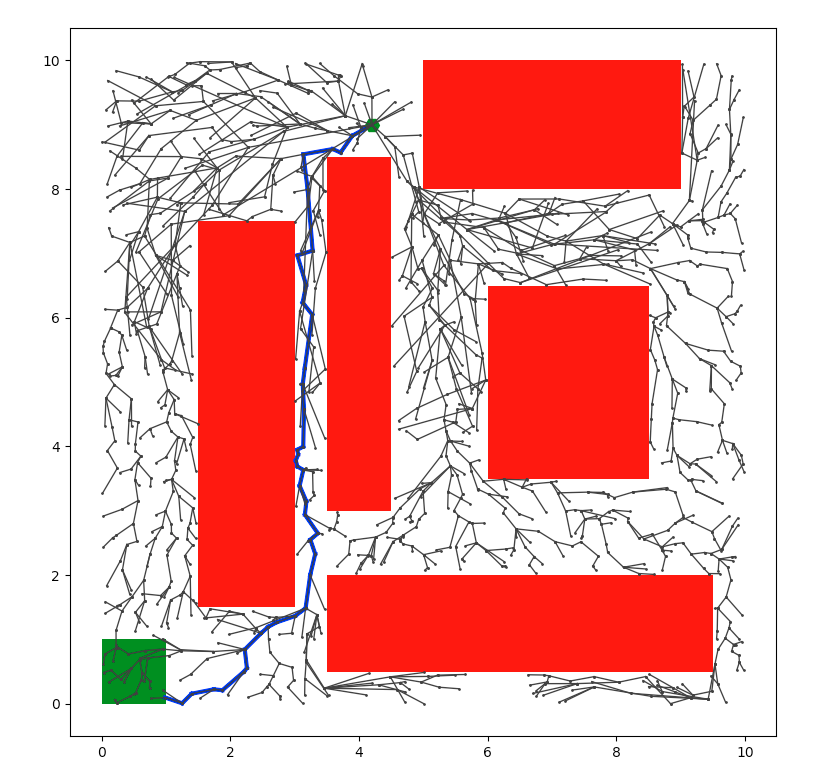
\includegraphics[scale=0.36]{./figures/fmt-2000-nodes}
    \caption[FMT* Example]{Example of a tree generated by \gls{fmt} using 2000 nodes. The initial state is shown at the top center as a green hexagon, the goal region lies in the bottom left and is shown in green, and obstacles are represented by red rectangles. The optimal path is highlighted in blue. This example does not use any dynamic model, so the cost function is simply the Euclidean distance.}
\label{fig:fmt_example}
\end{figure}

In more detail, \texttt{kinoFMT} takes as input an initial state, $x_{init}$, and goal region, $X_{goal}$, the state space, $\mathbb{X}$, the number of nodes to sample, and a cost threshold, $Jth$. The \texttt{Sample} function uniformly samples the entire state space\footnote{The \gls{fmt} algorithm specifies that samples are taken only from the free space (i.e., not including obstacles,) however, sampling from the entire state space allows for a much more general motion planning framework, as discussed in \autoref{chap:quad:rtmp}.} (usually with some samples selected directly from the goal region) and stores these sampled states in $\V$ along with $x_{init}$ (line~\ref{fmt:V}). 
The set $W$ contains unexplored nodes, and the set $H$ contains the nodes forming the frontier of expansion of the tree, which initially includes only $x_{init}$ (line~\ref{fmt:WH}). 
Every iteration, the least-cost node $z \in H$ becomes the pivot about which expansion occurs ({lines~\ref{fmt:z1},~\ref{fmt:z2}}). 
With the pivot known, we define $X_{near}$ to be the set of unexplored nearest nodes in the forward-reachable set of $z$ ({lines~\ref{fmt:loopz1}--\ref{fmt:loopz2}}). 
Then, for each element $x \in X_{near}$, define $Y_{near}$ to be the set of nodes in the frontier that are also in the backward-reachable set of $x$ ({lines~\ref{fmt:loopx1}--\ref{fmt:loopx2}}). 
The least-cost state $y_{min}$ is then found from the set of all $y \in Y_{near}$, where the cost is determined to be the sum of the cost of reaching $y$ (along its unique path from $x_{init}$) and the cost to travel from $y$ to $x$, recalling that $y$ is in the backward-reachable set of $x$ (line~\ref{fmt:dynprogram}). This is the dynamic programming step, where we try to minimize the cost-to-come and the cost-to-go. 
Once the cost minimizer is found, a collision check is performed (line~\ref{fmt:col}), and if a collision is detected along the transition from $y_{min}$ to $x$, then the algorithm simply discards this iteration and proceeds to the next. Otherwise, the edge (transition) is added to the tree, the newly connected node's cost is updated and the node is added to the frontier set, $H$, and it is simultaneously removed from the set of unexplored nodes, $W$ ({lines~\ref{fmt:col1}--\ref{fmt:col2}}). 
Once the for-loop has iterated through the entire set of forward-reachable nodes, $X_{near}$, the pivot, $z$, is removed from the frontier and the procedure repeats until either the frontier is empty, at which point ``Failure'' is returned ({lines~\ref{fmt:empty1}--\ref{fmt:empty2}}), or until $z$ lies within the goal region, at which point the algorithm terminates. 
The \texttt{Path} function simply returns the optimal path, that is, the unique path from $x_{init}$ to the final least-cost goal state, $z$.

A diagram illustrating the addition of a single transition using \gls{fmt} is provided in \autoref{fig:fmt_diagram}. In part $\text{a)}$ of the diagram, of the two nodes in the frontier, $H$, the one with least cost is selected as $z$. For this simple example, distance is used as the cost with a search radius of $J_{th}$, and three unvisited nodes are found to lie within this distance from $z$. These are the nodes belonging to $X_{near}$. The algorithm will iterate through all three nodes in $X_{near}$, but we focus on one for this example. In $\text{b)}$, we add all nodes whose search radius includes node $x$ to $N_x^{in}$. This set is not necessarily equivalent to the set of all nodes within the search radius of $x$; for non-symmetric cost functions, this distinction could have a significant impact (e.g., the \texttt{kinoFMT} algorithm). In $\text{c)}$, of the nodes in $N_x^{in}$, only those that are also in $H$ are included in the set $Y_{near}$. For each node $y \in Y_{near}$, the cost of each, $y.cost + \texttt{Cost}(\overline{y \to x})$, is computed and the least-cost node, $y_{min}$, is determined. Provided there is no collision when connecting $y_{min}$ to $x$, the edge is added to the tree and $x$ is added to the set $H$. Once this entire process is repeated for every $x \in X_{near}$, the next iteration begins with a new least-cost frontier node $z$, or returns ``Failure'' if $H$ is empty.

\begin{figure}[!ht]
    \vspace*{4mm}
    \hspace*{8mm}
    \centering
    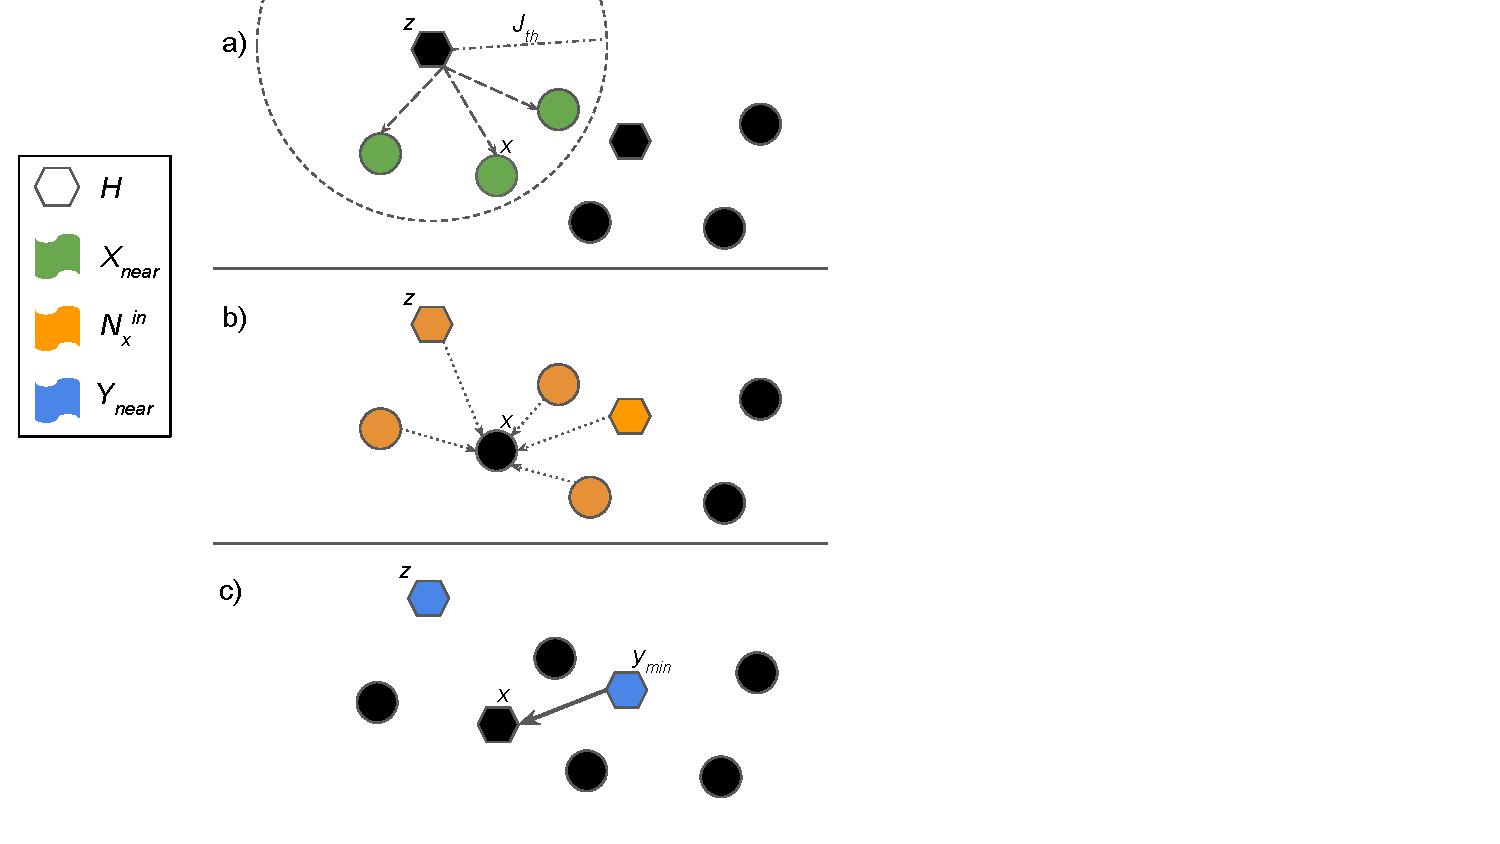
\includegraphics[scale=0.89]{./figures/fmt_diagram}
    \caption[FMT* Diagram]{
        Illustration of the \gls{fmt} algorithm.
    }
\label{fig:fmt_diagram}
\end{figure}
